\section{沿固定失败起点路径观察}
\label{sec:process}

\subsection{固定分析集合、首次通过停止与退出}
\label{subsec:process-cohort}
现在回到第~\ref{subsec:segment-rule}~节和第~\ref{subsec:failure-cohort}~节定义的高置信重建：367 条边形成 262 个完整连续片段，从中选取起点明确失败的 230 个片段，得到涉及 182 个任务的固定分析集合。选取起点与在首次通过处停止观察是两项操作；不会仅因为后来的记录属于同一任务，就把它接入原路径。

按照第~\ref{sec:process-theory}~节的定义，第 1 步是从失败起点到另一送审候选的第一次合格转移，其结果是后一个候选获得的审核标签。随后每一步也都是一次这样的送审版本转移。路径在第一次记录通过或允许的链条结束时停止，以先发生者为准。230 条路径总共贡献 329 个实际观察的步骤。每个步骤及其结果构成一条\emph{合格步骤记录}，传统上也称为\emph{风险行}。“处于风险中”在这里仅指仍有资格记录\emph{首次}通过。

这里有两种终态。206 条路径在链条结束之前记录通过，另外 24 条到达链条边界时尚未出现这种通过。针对本节的问题，退出是已经观察到的终态，不是把某个未知结果悄悄填成“不通过”。它描述的是这条分析路径在哪里结束，不证明任务被放弃、不证明未来候选都会失败，也不说明应该把别处的最终通过添加到原路径。

如果问题变了，对退出的处理也会变。如果我们问的是“\emph{同一种机制假如一直运行下去}，这个任务还要多久才通过”，退出之后的结果就是未观察的。把这样的记录称为删失，并不会让缺失的后续结果变得已知；还需要额外假设，把假想的持续过程与已观察路径联系起来。本报告不估计这种假想等待时间。

\subsection{逐步计数、风险集与累计比例}
\label{subsec:risk-counts}
第 1 步，全部 230 条失败起点路径都具有观察资格。其中 167 条通过，18 条尚未通过就结束，45 条继续进入第 2 步：
\[
230=167+18+45.
\]
第 2 步，只剩下这 45 条继续的路径。其中 29 条通过，4 条退出，12 条继续：
\[
45=29+4+12.
\]
第二个分母是 45，因为此时所问的是到达第 2 步的路径。它不是又抽取了 230 条路径，也不是把全部任务多修改一次之前和之后作比较。表~\ref{tab:process-counts}~把同样的计数一直列到最后一个已观察步骤。

\begin{table}[htbp]
\centering
\caption{固定的 230 条路径。每一行把到达该步骤的路径分为通过、退出或继续，三类互不重叠。}
\label{tab:process-counts}
\small
\begin{tabular}{rrrrr}
\toprule
步骤 & 合格路径 & 通过 & 退出 & 继续 \\
\midrule
1 & 230 & 167 & 18 & 45 \\
2 & 45 & 29 & 4 & 12 \\
3 & 12 & 1 & 0 & 11 \\
4 & 11 & 5 & 0 & 6 \\
5 & 6 & 2 & 1 & 3 \\
6 & 3 & 0 & 0 & 3 \\
7 & 3 & 0 & 0 & 3 \\
8 & 3 & 0 & 0 & 3 \\
9 & 3 & 0 & 0 & 3 \\
10 & 3 & 0 & 0 & 3 \\
11 & 3 & 1 & 0 & 2 \\
12 & 2 & 1 & 0 & 1 \\
13 & 1 & 0 & 0 & 1 \\
14 & 1 & 0 & 0 & 1 \\
15 & 1 & 0 & 0 & 1 \\
16 & 1 & 0 & 0 & 1 \\
17 & 1 & 0 & 1 & 0 \\
\midrule
各步骤相加 & 329 & 206 & 24 & --- \\
\bottomrule
\end{tabular}
\end{table}

为了给所有步骤统一记号，令 $n_j$ 表示第 $j$ 步的合格路径数，$d_j$ 表示这一步通过的路径数，$c_j$ 表示这一步未通过后退出的路径数。于是，
\begin{equation}
 n_j=d_j+c_j+n_{j+1}.
 \label{eq:cohort-conservation}
\end{equation}
这是计数恒等式，不是拟合得到的模型。组成 $n_j$ 的那一组路径，叫作第 $j$ 步的\emph{风险集}。它的缩小可由记录通过数和退出数解释，不需要先假设通过概率恒定。

另外两个有用的累计量始终使用\emph{起初的}分母 230：
\begin{align}
 F_P(j)&=\frac{d_1+\cdots+d_j}{230},
 &F_X(j)&=\frac{c_1+\cdots+c_j}{230}.
 \label{eq:finite-incidences}
\end{align}
$F_P(j)$ 表示原始路径中截至第 $j$ 步已经通过的比例；$F_X(j)$ 表示截至这一步尚未通过就退出的比例。下标 $P$ 对应通过，$X$ 对应退出。它们是累计比例，也称累计发生比例。剩余比例为 $n_{j+1}/230$，所以这三个比例相加等于 1。在最后一个已观察步骤，
\[
 F_P(17)=206/230=89.57\%,\qquad
 F_X(17)=24/230=10.43\%.
\]
由于退出本来就是两种记录终态之一，计算这些有限路径的比例，不需要假设退出与未来成功彼此独立。

把一条路径直到通过或退出为止的合格转移次数，叫作它的\emph{已观察长度}。全部长度加起来为 329，因此平均长度为 $329/230=1.4304$ 次转移。短路径既可能很快通过，也可能很快退出；这个数字不是最终成功所需编辑次数的平均值。

\subsection{首步和后续步骤的比例具有不同构成}
\label{subsec:first-later}
全部首次步骤共有 $167/230=72.61\%$ 记录通过。把步骤编号为 2 或更大的记录合并，得到 $39/99=39.39\%$。分母 99 来自表~\ref{tab:process-counts}~中各个后续步骤合格数的相加，不是 99 条不同路径，更不是 99 个独立任务。一条长路径会贡献多条后续记录。“后续减首次”的差为
\[
100\left(\frac{39}{99}-\frac{167}{230}\right)=-33.21
\quad\text{个百分点}.
\]
这个数描述的是两组已经观察到的记录，不是把同一批任务全部强制多修改一次之后会出现的变化。

为了说明这些摘要在一个参考抽样模型下会如何波动，我们以任务为整体，从 182 个任务中有放回抽样，共重复 20,000 次，固定随机种子为 20260906。每次抽中一个任务，都保留它的全部原始路径及合格步骤记录，再利用汇总计数重新计算相应比例。重抽样结果的第 2.5 和第 97.5 百分位数构成表~\ref{tab:process-estimates}~中的 95\% 任务整群参考区间。这样保留了任务内部记录的依赖结构，但没有证明不同任务相互独立，也没有纠正历史选择机制。第~\ref{subsec:cluster-resampling}~节解释了这类参考区间的含义。

\begin{table}[htbp]
\centering
\caption{已观察摘要及 95\% 任务整群百分位参考区间。百分点差是两个比例相减；已观察长度以送审版本转移为单位。}
\label{tab:process-estimates}
\small
\begin{tabularx}{\linewidth}{Yrr}
\toprule
所计算的量 & 估计值 & 参考区间 \\
\midrule
首次步骤通过比例 & $72.61\%$ & $[66.40,78.60]\%$ \\
后续步骤通过比例 & $39.39\%$ & $[24.84,65.71]\%$ \\
后续减首次，单位为百分点 & $-33.21$ & $[-48.39,-7.49]$ \\
固定路径退出之前通过的比例 & $89.57\%$ & $[85.40,93.53]\%$ \\
到通过或退出的平均已观察长度 & $1.4304$ & $[1.2271,1.6955]$ \\
\bottomrule
\end{tabularx}
\end{table}

这些量是汇总任务计数之后的比率，不是无论一个任务贡献多少路径或记录，都给它相同权重的平均值。因此，它们与第~\ref{sec:statistics}~节的任务等权修改边分析在加权方式上不同。后续步骤的区间较宽，是因为这些记录数量有限，而且很不均匀地分布在任务之间。对于已经完整枚举的档案，表中比例除四舍五入外都是精确描述；区间讨论的是在任务独立、可交换、记录选择机制相同等条件下，假想重复抽样的波动。这些条件并没有由历史档案本身得到确认。

\begin{figure}[htbp]
\centering
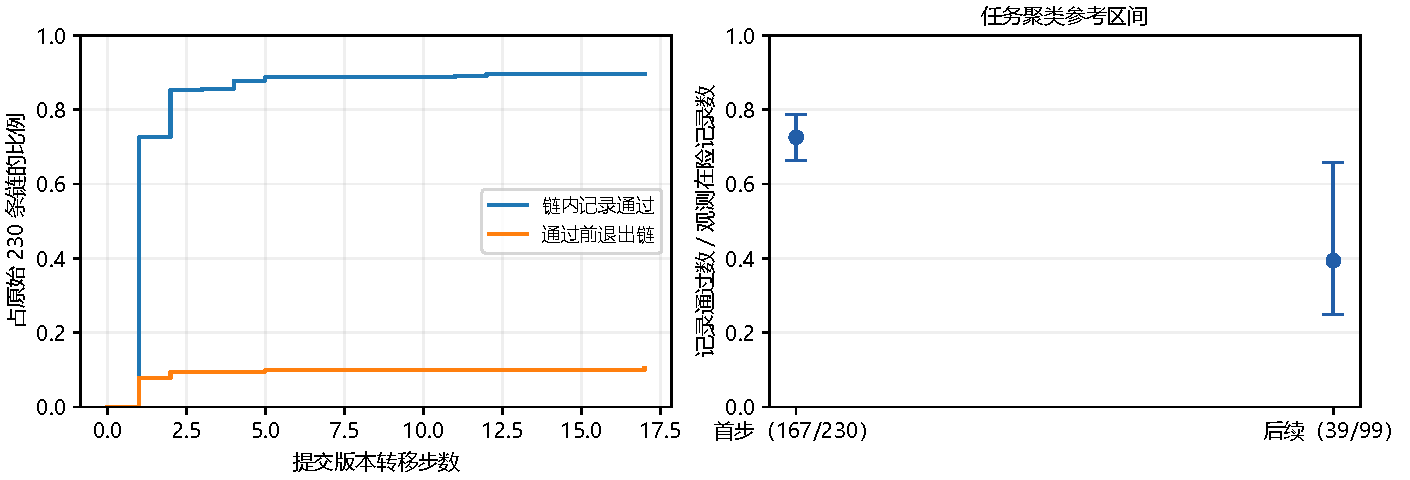
\includegraphics[width=\linewidth]{../figures/process_profile_zh.pdf}
\caption{同一组过程信息的图示。左侧为原始 230 条路径中的累计通过和退出比例；右侧为首次与后续已观察步骤的通过比例及任务整群百分位参考区间。图描述审核记录路径，不估计多编辑一次的效果。}
\label{fig:process}
\end{figure}

\begin{samepage}
\subsection{两组对数赔率模型及其系数}
\label{subsec:two-group}
过程模型比较首步和后续步骤两组记录的通过均值。使用对数赔率尺度，


\[
\operatorname{logit}(r)=\log\left(\frac{r}{1-r}\right),
\qquad
r=\frac{\exp(u)}{1+\exp(u)}\quad\text{当 }u=\operatorname{logit}(r).
\]
\end{samepage}
结果变量针对实际观察到的合格记录，两组可以具有不同的任务构成。

用 $s$ 给任务编号，用 $e$ 给同一任务中的不同路径编号，再用 $j$ 给一条路径内的步骤编号。对于一条已经观察到的合格记录，如果结果为记录通过，就令 $Y_{sej}=1$；否则令 $Y_{sej}=0$。再令 $L_j$ 表示是否属于后续步骤：$j=1$ 时为 0，$j\ge2$ 时为 1。最后，用 $\mu_{sej}$ 表示相应已观察记录组中这个二元结果的平均值。拟合的方程为
\begin{equation}
 \operatorname{logit}(\mu_{sej})=\alpha+\beta L_j.
 \label{eq:process-two-group-model}
\end{equation}
$\alpha$ 是首次步骤的对数赔率，$\beta$ 是到了后续步骤时要加在这个对数赔率上的数。因此，$\exp(\beta)$ 是后续相对于首次的赔率比。方程只拟合两个组均值，没有为每个任务单独设定基线，也没有控制任务难度。

分析使用针对二元结果的\emph{广义估计方程}，以工作独立性方式计算，并采用任务聚类稳健协方差。\cite{statsmodelsgee} 在这个简单的两组情形中，拟合均值恰好就是两组实际比例。因此，可以直接用组内计数核对系数：
\begin{align*}
 \widehat\alpha&=\log(167/63)=0.974859,\\
 \widehat\beta&=\log(39/60)-\log(167/63)=-1.405642.
\end{align*}
首次步骤共有 63 条未通过记录，后续步骤有 60 条。把 $L_j=0$ 代入对数赔率的逆变换，得到 $0.726087$；把 $L_j=1$ 代入，得到 $0.393939$。对两者的对数赔率之差取指数，则有
\[
\exp(\widehat\beta)=\frac{39/60}{167/63}=0.2452.
\]
这是两个已观察记录组的赔率比，不是修改的因果效果估计。

\subsection{任务聚类协方差与参考检验}
\label{subsec:robust-covariance}
来自同一个任务的多条记录可能共享候选历史、要求与审核条件。把 329 行全都当成互不相关的观察，会忽略这种结构。协方差按任务聚类，以处理任务内部依赖；两个拟合比例保持不变。

“工作独立性”是一种计算选择的名字，不是认为连续提交实际上独立的研究发现。这个修正也不会让不同任务变得独立：共享依赖、模型、规则或收集批次都可能使任务相互关联。聚类处理更没有消除任务难度，也没有消除哪些路径能够到达后续步骤的选择机制。

得到的 $\widehat\beta$ 的稳健标准误为 $0.413295$。近似的 95\% 瓦尔德区间使用正态参照与任务聚类协方差。在对数赔率尺度上，
\[
-1.405642\ \pm\ 1.96(0.413295)
\approx[-2.215685,-0.595599].
\]
对两个端点取指数，得到赔率比区间 $[0.1091,0.5512]$。把系数除以标准误，约得 $-3.4011$；与标准正态参考分布比较，得到名义上的双侧 $p$ 值 $0.0006712$。这里的原假设是 $\beta=0$，等价于首次和后续的拟合均值相同，或赔率比为 1。和第~\ref{sec:statistics}~节的检验一样，这是以指定条件为前提的参考计算，不检验数学语义正确性。

协方差还使用各任务的贡献独立重建过，与软件计算的最大绝对差为 $2.5\times10^{-16}$；独立复核也复现了按任务重抽样的结果。这检查的是指定输入和公式的计算是否一致，不认证记录选择机制，更不建立观察关联的因果解释。

作为对照，如果强制只使用一个共同均值，便得到汇总比例 $206/329=0.626140$。对于 $n$ 条记录中的 $d$ 次通过，独立伯努利工作似然为
\[
 \mathcal L(r)=r^d(1-r)^{n-d},\qquad 0<r<1.
\]
令\emph{工作对数似然} $\ell(r)=\log\mathcal L(r)$，则
\[
 \ell(r)=d\log r+(n-d)\log(1-r),\qquad
 \ell'(r)=\frac d r-\frac{n-d}{1-r}.
\]
令导数等于零，得到 $d(1-r)=(n-d)r$，所以 $r=d/n$。当通过和未通过都出现时，二阶导数为负，因此这里是最大值。代入已观察的 $d=206,n=329$，就得到上面的汇总比例。

这是\emph{独立伯努利工作似然}，不是依赖形式尚未指定的整个任务过程的完整联合似然。把这个方便的函数最大化，不会证明它所假定的独立性。另外，限制 $\beta=0$ 只是在比较两个已观察记录组的均值。命题~\ref{prop:stopping}~中的恒定条件概率，要求在每一种合格过去历史之后都相等，这是强得多的陈述。这个两组检验既不认证，也不能全面检验那个更强的模型；尤其不能据此说多做一次修改会导致成功概率降低。

\subsection{为什么选取有后续观察的任务会改变首步组}
\label{subsec:later-selection}
182 个任务中，只有 39 个任务贡献后续步骤记录。如果看完整段历史之后再选出这些任务，它们的首次步骤有 61 条记录，其中 12 条通过，即 $19.67\%$。此时，后续记录的 $39.39\%$ 看起来高于选中任务的首次比例；而在与完整首次组的 $72.61\%$ 比较时，它又更低。算术没有错，但是人群构成变了。

把这 61 条首次记录拆开，原因就清楚了。其中 45 条属于后来确实继续的路径。按照第一次通过就停止的规则，这些首次步骤必然全部未通过，所以它们必然是 $0/45$。其余 16 条是这 39 个任务中\emph{另外一些路径}的首次步骤，其中 12 条通过。因此，$61=45+16$，而 $12=0+12$。因为任务有后续观察才把任务选进来，实际上就保留了许多“为了能够继续，首次必须未通过”的记录。

相对于第 1 步，这个筛选使用了未来信息。它不是把同一批任务平衡地分配到两种修改次数下进行比较。方向反转本身不能辨识改善机制、难度机制或因果效果。给它套用某个统计悖论的名字，也不能代替对分母的解释。

作为一个有限的影响检查，每次删去一个任务重新计算，后续减首次的差落在 $-36.07$ 至 $-23.57$ 个百分点之间，赔率比落在 $0.2156$ 至 $0.3593$ 之间。删去任何单个任务都没有使汇总关联反向，但这不解决任务间依赖或档案选择问题。加入中置信度修改边还可能重新连接路径，改变失败起点人群本身。那属于不同人群的敏感性问题；本节继续使用原始高置信度路径。

因此，过程结果作出的结论有明确范围：描述指定历史重建中，记录通过与退出何时发生，并量化记录结果与已观察过程位置之间的关联。它不估计多编辑一次的因果价值，不估计数学真值的概率，也不估计未观察继续策略下的等待时间。随附的冻结输入和脚本让这些具体计算可以复现，没有增加新的审核实验。
